%%=============================================================================
%% Contextanalyse en asset inventory
%%=============================================================================

\chapter{\IfLanguageName{dutch}{Contextanalyse en asset inventory}{Context analysis and asset inventory}}%
\label{ch:contextanalyse}

Dit hoofdstuk beschrijft de concrete beginsituatie van de onderzochte IP-camerainfrastructuur bij meubelzaak De Rore. Waar Hoofdstuk~\ref{ch:stand-van-zaken} het theoretische kader schetst en Hoofdstuk~\ref{ch:methodologie} de onderzoeksaanpak toelicht, vormt dit hoofdstuk de feitelijke basis voor de verdere risicoanalyse. De focus ligt op de aanwezige assets, hun netwerkpositie, de belangrijkste datastromen en de manier waarop het systeem in de praktijk wordt beheerd.

De contextanalyse is bewust beschrijvend opgevat. Het doel is in deze fase nog niet om alle vaststellingen definitief te beoordelen, maar om de technische en organisatorische context voldoende nauwkeurig vast te leggen. De prioritering van risico's gebeurt pas in Hoofdstuk~\ref{ch:risicoanalyse}; de technische validatie van geselecteerde hypothesen volgt in Hoofdstuk~\ref{ch:validatie}.

\section{\IfLanguageName{dutch}{Doel en afbakening van de contextanalyse}{Objective and scope of the context analysis}}%
\label{sec:context-doel}

De contextanalyse heeft als doel om een reproduceerbaar overzicht te creëren van de camerainfrastructuur die binnen de casusomgeving aanwezig is. Daarbij worden niet alleen de camera's zelf geïnventariseerd, maar ook de centrale recorder, netwerkcomponenten, beheerhost, gebruikte software, bekende IP-adressen, beheerpraktijken en relevante trust boundaries. Deze inventaris vormt de basis voor de latere risicoanalyse en bepaalt welke onderdelen in de gecontroleerde validatiefase verder onderzocht worden.

De analyse is afgebakend tot de IP-camerainfrastructuur van De Rore en de netwerkpaden die nodig zijn voor beheer, opslag, live view en eventuele toegang op afstand. Andere bedrijfsprocessen en IT-systemen vallen enkel binnen de scope wanneer zij relevant zijn voor de netwerkpositie of het risico op laterale beweging. De contextanalyse omvat dus geen algemene pentest van de volledige bedrijfsomgeving, maar een gerichte inventarisatie van de cameraketen en haar koppeling met het interne netwerk.

De gebruikte informatiebronnen bestaan uit de beschikbare installatiefiche, de checklist, de doorgestuurde IP-lijst, veldobservaties, screenshots uit de beheeromgeving, passieve netwerkobservaties en een plattegrond met cameramarkeringen. Omdat bepaalde netwerkcomponenten niet volledig konden worden uitgelezen, worden sommige topologische vaststellingen in dit hoofdstuk als werkhypothese geformuleerd. Waar nodig wordt expliciet aangegeven welke elementen later verder gevalideerd worden.

\section{\IfLanguageName{dutch}{Organisatorische context van De Rore}{Organisational context of De Rore}}%
\label{sec:context-organisatorisch}

De Rore is een retailomgeving waarin camerabewaking wordt gebruikt voor veiligheid, diefstalpreventie en operationele opvolging. Het camerasysteem maakt daardoor deel uit van de dagelijkse werking van de winkel. De beelden worden lokaal opgeslagen op een centrale recorder en kunnen via beheersoftware worden geraadpleegd. De installatie werd oorspronkelijk geplaatst door een externe leverancier en is nadien niet structureel vernieuwd.

Binnen deze context is het beheer van de camerainfrastructuur beperkt formeel uitgewerkt. De beschikbare informatie wijst erop dat de toegang tot het systeem vooral praktisch georganiseerd is: een gedeelde beheeromgeving, lokale opslag op de recorder en gebruik van TruVision Navigator voor live view en raadpleging. Er is geen aanwijzing dat er een afzonderlijk, gedocumenteerd proces bestaat voor periodieke firmware-updates, accountcontrole, loggingopvolging of configuratieback-ups. Daardoor is de beveiliging van het systeem in sterke mate afhankelijk van initiële configuratiekeuzes en van de mate waarin toegang tot de beheeromgeving in de praktijk wordt beperkt.

De organisatorische context is belangrijk voor de interpretatie van de technische vaststellingen. In een KMO- of retailomgeving zijn beheerprocessen doorgaans pragmatischer ingericht dan in grotere organisaties met gespecialiseerde IT- of securityteams. Maatregelen die in latere hoofdstukken worden voorgesteld, moeten daarom niet alleen technisch correct zijn, maar ook uitvoerbaar blijven binnen de operationele realiteit van de winkel.

\section{\IfLanguageName{dutch}{Overzicht van de camerainfrastructuur}{Overview of the camera infrastructure}}%
\label{sec:context-infrastructuur}

De camerainfrastructuur bestaat uit een centrale TruVision NVR, meerdere TruVision-IP-camera's, minstens één managed PoE-switch en bijkomende TP-Link-netwerkcomponenten die een rol spelen in de bereikbaarheid tussen het beheersegment en het cameragerelateerde netwerk. De centrale recorder is geïdentificeerd als een TruVision NVR 21 van UTC Fire \& Security, gekoppeld aan het model TVN-2116-4TE. Het toestel ondersteunt zestien IP-kanalen en fungeert als centrale opslag- en beheercomponent voor de camerabeelden.

Volgens de beschikbare apparaat- en installatiegegevens zijn zestien camerakanalen aanwezig. Daarvan zijn veertien camera's operationeel en twee camera's defect. De NVR bevat lokale opslag, waarbij opgenomen beelden volgens een overschrijfprincipe worden bewaard: wanneer de opslagcapaciteit bereikt wordt, worden de oudste beelden automatisch overschreven door nieuwere opnames. De apparaatinfo vermeldt een opslagcapaciteit van 4 TB, terwijl de installatiefiche ook verwijst naar een opslagconfiguratie van 3 x 2 TB. Dat verschil wordt in dit hoofdstuk niet als kwetsbaarheid beoordeeld, maar wel als een aandachtspunt voor de volledigheid van de technische inventaris.


\begin{figure}[H]
         \centering
         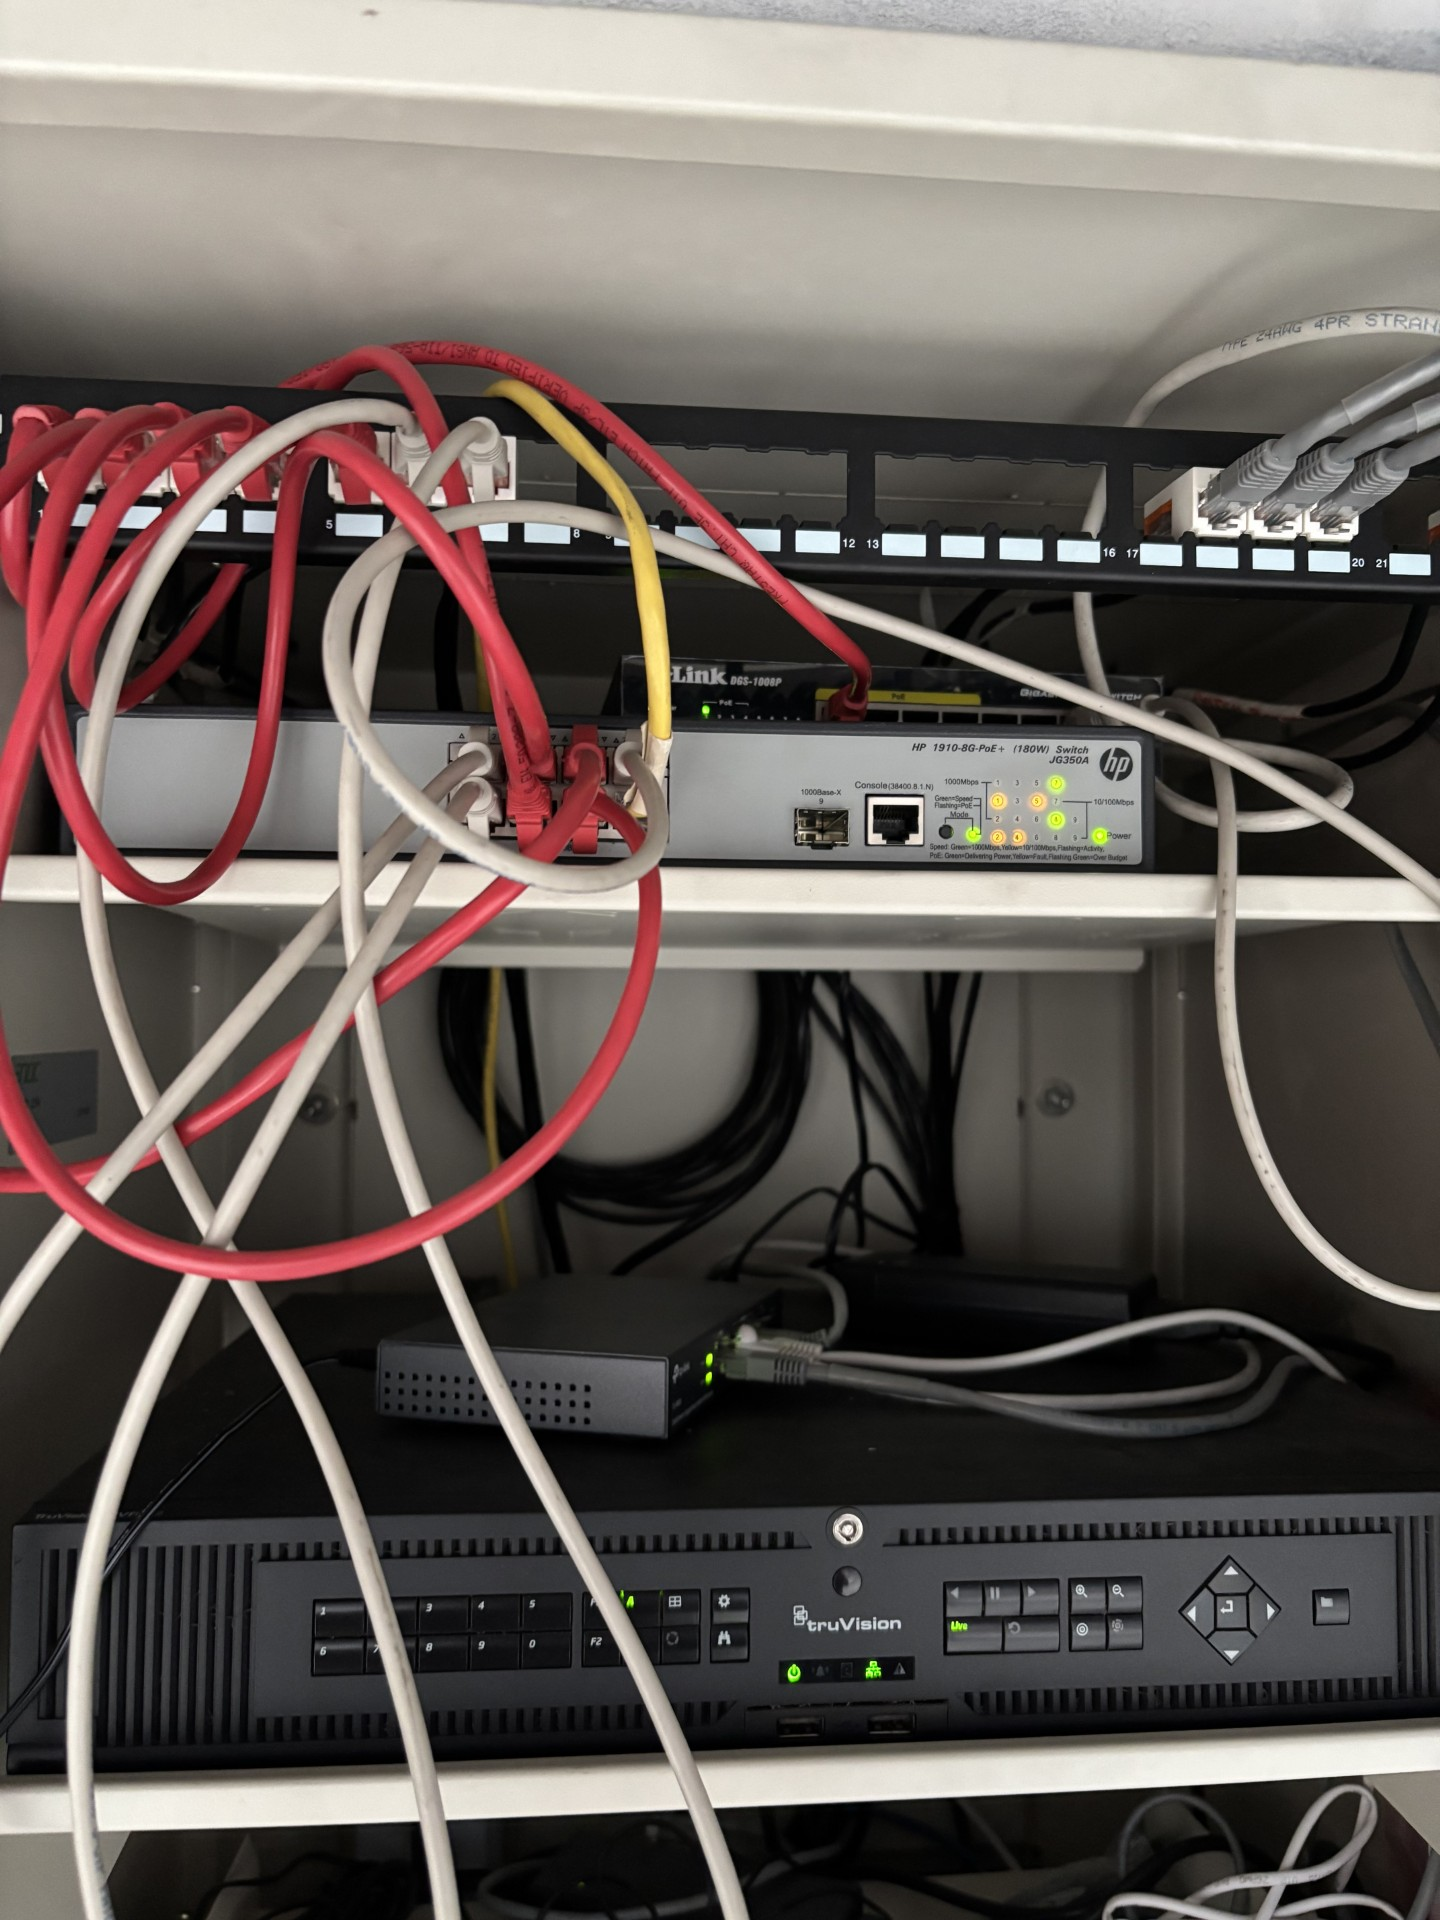
\includegraphics[width=.8\textwidth]{../Voorbereiding/Bewijsstukken/H1/foto_nvr_switch_opstelling}
         \caption[Opstelling van NVR en netwerkcomponenten]{Fysieke opstelling van de NVR en relevante netwerkcomponenten binnen de onderzochte omgeving.}
         \label{fig:opstelling-nvr-switch}
    \end{figure}

Tabel~\ref{tab:centrale-assets} geeft een samenvatting van de belangrijkste centrale componenten.

\begin{table}[H]
    \centering
    \small
    \caption[Overzicht van centrale componenten]{Overzicht van de belangrijkste centrale componenten binnen de camerainfrastructuur.}
    \label{tab:centrale-assets}
    \begin{tabular}{|p{.25\textwidth}|p{.65\textwidth}|}
        \hline
        \textbf{Component} & \textbf{Vaststelling} \\
        \hline
        NVR & TruVision NVR 21 / TVN-2116-4TE, centrale opslag- en beheercomponent voor maximaal zestien IP-kanalen. \\
        \hline
        Opslag & Lokale opslag op de NVR met overschrijfprincipe. Beschikbare documentatie vermeldt zowel 4 TB als een configuratie van 3 x 2 TB. \\
        \hline
        Camera's & Zestien camerakanalen, waarvan veertien operationeel en twee defect. \\
        \hline
        Beheersoftware & Live view en beheer gebeuren via TruVision Navigator 6.0 en via beschikbare beheerinterfaces. \\
        \hline
        Switch & Minstens één HP 1910-8G-PoE+ managed switch is aanwezig in de cameraketen. \\
        \hline
        Tussencomponenten & TP-Link-componenten zijn bereikbaar op 10.0.0.150 en 192.168.0.212 en spelen vermoedelijk een rol in routing, bridging of toegang tot het cameradomein. \\
        \hline
    \end{tabular}
\end{table}

De camera-inventaris is opgebouwd op basis van de beschikbare installatiedocumentatie, de NVR-weergave en de aanvullende fysieke koppeling met de plattegrond. Tabel~\ref{tab:camera-inventaris} geeft de gekende camera's en IP-adressen weer.

\begin{table}[H]
    \centering
    \small
    \caption[Camera-inventaris met IP-adressen]{Voorlopige camera-inventaris met gekende locaties en IP-adressen.}
    \label{tab:camera-inventaris}
    \begin{tabular}{|p{.18\textwidth}|p{.46\textwidth}|p{.24\textwidth}|}
        \hline
        \textbf{Camera} & \textbf{Naam / plaats} & \textbf{IP-adres} \\
        \hline
        Camera 1 & Toonzaal, tweede gang & 192.168.0.18 \\
        \hline
        Camera 2 & Toonzaal, eerste gang & 192.168.0.17 \\
        \hline
        Camera 3 & Toonzaal, tweede gang & 192.168.0.14 \\
        \hline
        Camera 4 & Toonzaal, tweede gang & 192.168.0.16 \\
        \hline
        Camera 5 & Toonzaal, tweede gang & 192.168.0.15 \\
        \hline
        Camera 6 & Toonzaal achter links & 192.168.0.10 \\
        \hline
        Camera 7 & Toonzaal achter links & 192.168.0.11 \\
        \hline
        Camera 8 & Toonzaal achter rechts & 192.168.0.12 \\
        \hline
        Camera 9 & Toonzaal achter rechts & 192.168.0.13 \\
        \hline
        Camera 10 & Toonzaal vooraan, muurtje & 192.168.0.19 \\
        \hline
        Camera 11 & Inkom & 192.168.0.20 \\
        \hline
        Camera 12 & Magazijn, defect & 192.168.0.21 \\
        \hline
        Camera 13 & Buiten, buitensirene, defect & 192.168.0.22 \\
        \hline
        Camera 14 & Buiten, boven container & 192.168.0.23 \\
        \hline
        Camera 15 & Toonzaal vooraan midden & 192.168.0.25 \\
        \hline
        Camera 16 & Toonzaal splitsing vooraan en achteraan & 192.168.0.26 \\
        \hline
    \end{tabular}
\end{table}

Op basis van de aanvullende inventarisatie kunnen de cameramodellen als volgt worden samengevat. Camera 13 en 14 behoren tot het model TVC-M3245E-2M-P. Camera 11 en 12 behoren tot het model TVD-M3245E-ZM-P. De overige camera's behoren tot het model TVD-M2210W-4-P. Deze heterogene samenstelling is relevant voor de latere risicoanalyse, omdat verschillen in model, firmware, beheerinterface en protocolondersteuning het beheer complexer kunnen maken.


 \begin{figure}[H]
         \centering
         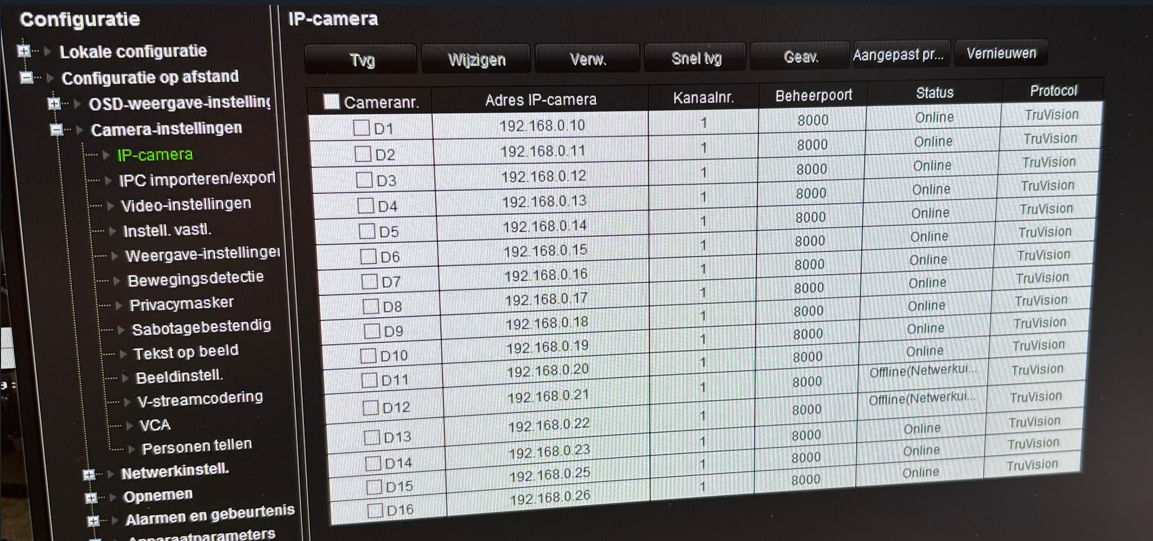
\includegraphics[width=\textwidth]{../Voorbereiding/Bewijsstukken/H1/screenshot_camera_overzicht}
         \caption[Camera-overzicht in de beheeromgeving]{Camera-overzicht in de beheeromgeving met IP-adressen en status per kanaal.}
         \label{fig:camera-overzicht}
     \end{figure}

% TODO FOTO/FIGUUR:
% Voeg hier of in de bijlage de plattegrond toe waarop de cameranummers zichtbaar zijn.
%
 \begin{figure}[H]
         \centering
         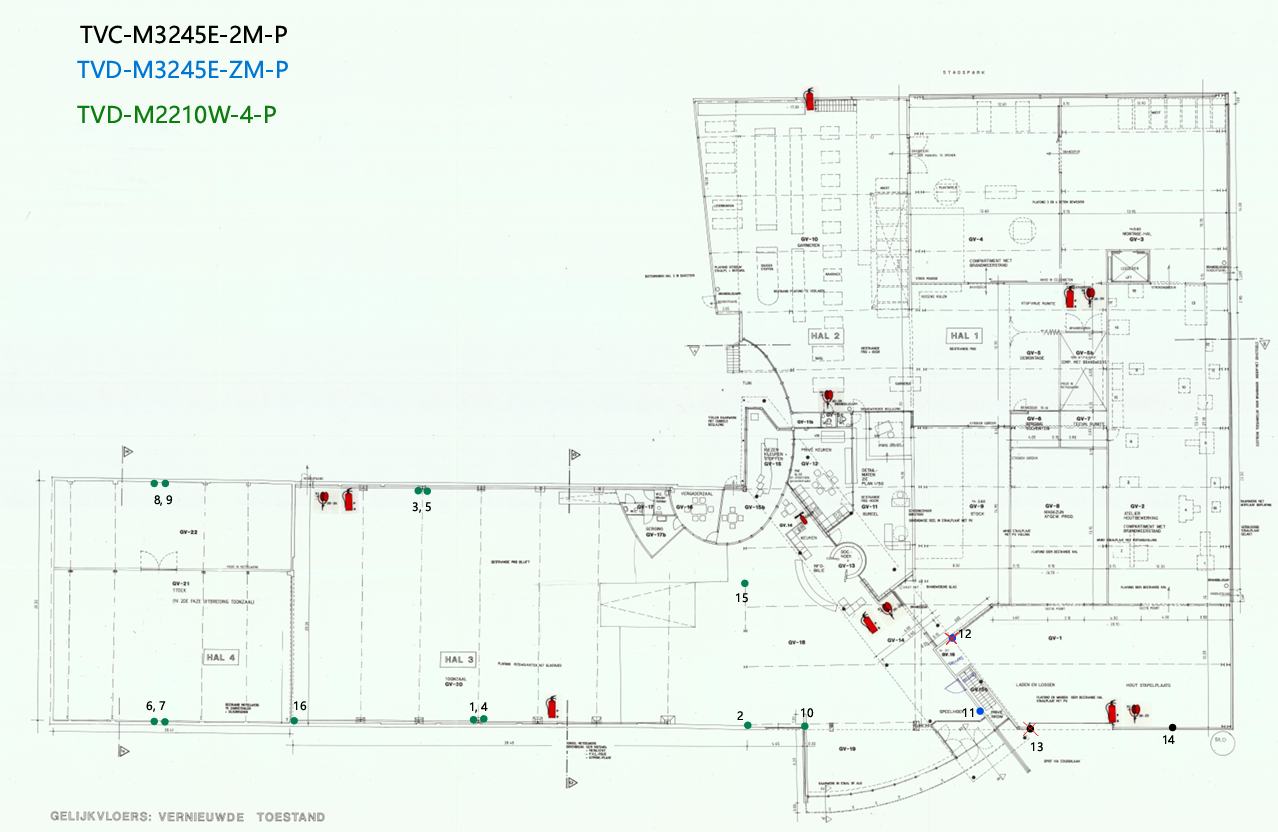
\includegraphics[width=\textwidth]{../Voorbereiding/Bewijsstukken/H1/plattegrond_cameranummers}
         \caption[Plattegrond met cameraposities]{Plattegrond van de winkelomgeving met aanduiding van de cameraposities en cameranummering.}
         \label{fig:plattegrond-cameras}
     \end{figure}

\section{\IfLanguageName{dutch}{Netwerkpositie en datastromen}{Network position and data flows}}%
\label{sec:context-netwerkpositie}

De initiële aanname dat de camerainfrastructuur zich in één volledig vlak netwerk bevond, moest tijdens de contextanalyse worden genuanceerd. De huidige werkhypothese is dat minstens twee IP-zones betrokken zijn: een beheer- of wifi-segment in de range 10.0.0.0/24 en een cameragerelateerd segment in de range 192.168.0.0/24. Tussen beide zones bevinden zich minstens één of meerdere TP-Link-componenten. De component op 10.0.0.150 fungeert daarbij als gateway of transitpunt vanuit het beheersegment, terwijl 192.168.0.212 als bijkomende downstream component of routed hop werd vastgesteld.

De NVR wordt in de beschikbare documentatie gekoppeld aan het lokale adres 10.0.0.60. De camera's bevinden zich volgens de inventaris hoofdzakelijk in de range 192.168.0.10 tot en met 192.168.0.26. Deze combinatie wijst erop dat de NVR, camera's en beheercomponenten niet zonder meer als één uniform subnet mogen worden geïnterpreteerd. Er is minstens sprake van een netwerkpad waarbij beheer- en camerazone via tussenliggende componenten met elkaar verbonden zijn. De exacte implementatie, bijvoorbeeld VLAN-segmentatie, routing of bridging, kon in deze fase nog niet volledig worden bevestigd.

Conceptueel kan de voorlopige netwerkpositie als volgt worden samengevat:

\begin{center}
    \begin{minipage}{0.9\textwidth}
        \centering
        Beheer-/wifi-segment \texttt{10.0.0.0/24}\\
        \textit{met o.a. testhost \texttt{10.0.0.156} en NVR \texttt{10.0.0.60}}\\[0.4em]
        $\downarrow$\\[0.4em]
        
        Router/default gateway op \texttt{10.0.0.150}\\[0.4em]
        $\downarrow$\\[0.4em]
        
        Gerouteerd of downstream pad richting \texttt{192.168.0.0/24}\\
        \textit{met waargenomen tussenliggende component \texttt{192.168.0.212}}\\[0.4em]
        $\downarrow$\\[0.4em]
        
        Cameradomein met camera-adressen \texttt{192.168.0.10} t.e.m. \texttt{192.168.0.26}\\
        \textit{IP-camera's, PoE-connectiviteit, streams en opnamefunctionaliteit}
    \end{minipage}
\end{center}

De belangrijkste datastromen binnen de cameraketen zijn videostreaming van de camera's naar de NVR, live view via TruVision Navigator, beheercommunicatie naar de NVR of tussenliggende beheerinterfaces, lokale opslag van videobeelden en eventuele export van beelden. De NVR bevindt zich volgens de beschikbare configuratiegegevens op \texttt{10.0.0.60}, terwijl de individuele camera's geadresseerd zijn binnen het bereik \texttt{192.168.0.10} tot en met \texttt{192.168.0.26}. De communicatie tussen deze componenten verloopt daardoor vermoedelijk via één of meerdere tussenliggende netwerkcomponenten, waaronder \texttt{10.0.0.150} en \texttt{192.168.0.212}. De exacte rol van deze componenten wordt in deze fase nog voorzichtig geïnterpreteerd als gateway-, transit- of downstreamfunctionaliteit.

Daarnaast vermelden de verzamelde configuratiegegevens historische of operationele mogelijkheden voor toegang op afstand via DynDNS, port forwarding en VPN. Deze vaststelling betekent niet automatisch dat individuele camera's rechtstreeks vanaf het internet bereikbaar zijn. In deze fase worden de camera's zelf niet als rechtstreeks internet-exposed beschouwd; de verdere analyse focust vooral op de NVR, de tussenliggende beheercomponenten en de afscherming van de beheerpaden.

Een bijkomende observatie is dat passief netwerkverkeer reeds nuttige inventarisinformatie kan vrijgeven. In de geanalyseerde netwerkcaptures werd onder meer vastgesteld dat de NVR met IP-adres \texttt{10.0.0.60} broadcast- of discoveryverkeer verstuurt waarin cameragerelateerde metadata zichtbaar wordt, waaronder camera-adressen in de \texttt{192.168.0.x}-range. Dit betekent niet dat de individuele camera's zelf rechtstreeks vanuit het onderzochte segment bereikbaar zijn, maar wel dat de NVR informatie over deze cameracomponenten zichtbaar maakt binnen het netwerkverkeer. Daarnaast waren in het onderzochte netwerk ook niet-cameragerelateerde discoverydiensten zichtbaar, zoals mDNS-, SSDP- en UPnP-verkeer van andere toestellen. Deze observatie suggereert dat een intern toestel relatief veel zichtbaarheid kan krijgen op componenten en services binnen de omgeving. De precieze beveiligingsimpact daarvan wordt verder behandeld in de risicoanalyse en validatiehoofdstukken.

\section{\IfLanguageName{dutch}{Beheerprocessen en configuratiepraktijken}{Management processes and configuration practices}}%
\label{sec:context-beheerprocessen}

De beheerpraktijk rond de camerainfrastructuur is beperkt formeel uitgewerkt. Zowel op de beheerhost als binnen de camerabeheeromgeving wordt gewerkt met een gedeeld adminaccount. Er zijn geen aanwijzingen dat er persoonlijke accounts, rollen of gescheiden rechtenprofielen worden gebruikt. Daardoor is er in de praktijk geen duidelijke scheiding tussen gewone raadpleging en administratief beheer. Wie toegang heeft tot de gedeelde beheeridentiteit, kan potentieel ook instellingen wijzigen of beheerfunctionaliteit gebruiken.

De standaardwachtwoorden werden aangepast, maar het gebruikte wachtwoord wordt in de contextanalyse als zwak beoordeeld omdat het kort is en sterk verbonden is aan de bedrijfscontext. Het wachtwoord zelf wordt om veiligheidsredenen niet in deze bachelorproef opgenomen. Daarnaast is geen multifactorauthenticatie aanwezig voor de beheeromgeving of voor eventuele toegang op afstand.

Ook het lifecyclebeheer van de infrastructuur is beperkt. De installatie dateert uit 2016 en de NVR draait op een oude firmwareversie. Er is geen formele update- of patchprocedure vastgesteld en updates worden niet periodiek uitgevoerd. Daardoor bestaat het risico dat bekende kwetsbaarheden in firmware of beheerinterfaces aanwezig blijven. In deze context is vooral de combinatie van verouderde componenten, zwakke toegangscontrole en beperkte segmentatie relevant.

Wat logging betreft, zijn op de recorder loginlogs en exportgerelateerde gebeurtenissen zichtbaar. De logging toont dus dat bepaalde acties worden geregistreerd, maar er is in deze fase nog geen bewijs dat logs actief worden opgevolgd, centraal worden bewaard of automatisch aanleiding geven tot waarschuwingen. Daardoor moet logging voorlopig worden gezien als een beperkte auditmogelijkheid, niet als een volwaardige detectie- en monitoringlaag.

\section{\IfLanguageName{dutch}{Eerste risico-observaties}{Initial risk observations}}%
\label{sec:context-eerste-risicos}

De contextanalyse levert een eerste reeks beveiligingsrelevante observaties op. Deze observaties vormen nog geen definitieve risicobeoordeling, maar geven wel richting aan de prioritering in Hoofdstuk~\ref{ch:risicoanalyse}.

Een eerste observatie is dat de toegangscontrole sterk afhankelijk is van één gedeelde adminidentiteit. Hierdoor ontbreken individuele verantwoordelijkheid, functiescheiding en fijnmazige toegangscontrole. Dit verhoogt de kans dat beheerrechten ruimer verspreid zijn dan noodzakelijk en bemoeilijkt de reconstructie van handelingen achteraf.

Een tweede observatie is dat de netwerkstructuur niet volledig transparant is. Er zijn aanwijzingen voor minstens twee IP-zones en meerdere tussenliggende componenten, maar de exacte rol van VLAN's, routing en bridging is nog niet volledig bevestigd. Dit maakt het moeilijk om op basis van documentatie alleen te bepalen welke systemen elkaar kunnen bereiken en waar de effectieve trust boundaries liggen.

Een derde observatie is dat de infrastructuur legacykenmerken vertoont. De NVR en installatie zijn oud, updates worden niet structureel uitgevoerd en sommige componenten of camera's zijn defect of niet volledig gedocumenteerd. Daardoor ontstaat een verhoogde afhankelijkheid van bestaande configuraties, terwijl de actuele beveiligingsstatus niet automatisch gegarandeerd is.

Een vierde observatie betreft de zichtbaarheid van beheer- en discoveryinformatie binnen het interne netwerk. De aanwezigheid van webinterfaces op tussenliggende componenten, broadcastverkeer van de NVR en discoveryverkeer van andere toestellen wijst op een relatief brede interne zichtbaarheid. Dit is vooral relevant wanneer een aanvaller of onbevoegde gebruiker al toegang heeft tot het interne of beheergerelateerde netwerk.

Ten slotte blijft de exacte afscherming van toegang op afstand een belangrijk aandachtspunt. De historische configuratie vermeldt DynDNS, port forwarding en VPN, maar in deze fase wordt nog niet geconcludeerd dat individuele camera's rechtstreeks publiek bereikbaar zijn. De verdere validatie moet daarom vooral nagaan welke beheerpaden effectief bereikbaar zijn en of die voldoende afgeschermd zijn.

Samengevat toont dit hoofdstuk dat de belangrijkste aandachtspunten niet voortkomen uit één afzonderlijke kwetsbaarheid, maar uit de combinatie van gedeelde accounts, zwak wachtwoordbeheer, beperkte lifecycleprocessen, onvolledig gevalideerde netwerksegmentatie, zichtbare beheerpaden en beperkte loggingopvolging. Deze vaststellingen worden in het volgende hoofdstuk vertaald naar een geprioriteerde risicoanalyse en een afgebakende set onderzoekshypothesen.
